\chapter{非线性光学性质的Wannier插值计算方法}

非线性光学效应在现代光学和现代凝聚态物理中起着非常重要的作用\cite{boyd-nlo}。非线性光学材料在很多领域都有非常重要的实际应用,尤其是激光科学技术领域\cite{nurmikko-compact,kanai_generation_2004,boyd-nlo}。非线性光学材料可以通过频率转换,将现有的激光转换到远红外或者远紫外频率\cite{nurmikko-compact,kanai_generation_2004}。尽管非线性光学研究已经有了半个世纪以上的历史,但是对新奇的非线性光学效应的探索仍然没有停止\cite{young2012,young2012_2,tan2016,morimoto2016,morimoto2016prb,rangel_giant_2016,cook_design_2017,wu_giant_2017}。近几年来,人们逐渐开始研究贝里相位和拓扑效应在非线性光学中的效应\cite{xiao2010,hasan2010,qi2011}。重要的是,最近的理论工作揭示了包括位移电流,倍频效应,光伏霍尔效应等等效应都和拓扑相关的物理量如贝里相位和贝里曲率有关系\cite{morimoto2016,morimoto2016prb}。除此之外,实验和理论都证实了在拓扑材料中的非线性光学效应非常显著\cite{tan2016,wu_giant_2017}。在这样的背景下,研究非线性光学现象中的拓扑效应就成为了非常重要的课题。

在材料科学领域,第一性原理方法非常有效,不可替代。第一性原理方法能够在不引入任何经验参数的情况下计算材料的各种性质。现如今,人们多次使用第一性原理方法计算非线性光学效应\cite{sipe_second-order_2000,young2012,rangel_giant_2016,cook_design_2017}。但是,这些方法计算量都非常地大,布里渊区的积分需要极密的$k$点。另外一方面,第一性原理生成的波函数的相位不确定性,如果没有得到很好的处理,将无法计算贝里相位和贝里相位的导数。这个问题被称为相位问题。要解决这些问题,人们需要新的计算非线性光学效应的方法。最近,基于Mazari等人提出的最大局域化Wannier函数方法\cite{marzari_maximally_1997,marzari2012},Wannier插值方法被用来计算各种各样的物理量,包括反常霍尔电导,轨道磁矩等等\cite{wang_textitab_2006,yates_spectral_2007,lopez_wannier-based_2012}。这些计算采用一阶微扰来解决相位问题。Wannier插值方法计算量很小,并且可以和绝大部分第一性原理计算方法接口,包括密度泛函理论,杂化泛函和$GW$方法。但是,据我们所知,并没有人尝试用Wannier插值方法计算非线性光学效应。


我们在这里将Wannier插值方法推广,用以计算非线性光学效应。这个方法通过二阶微扰构建了一个平滑的相位规范,可以准确计算任何$k$点的波函数的导数和二阶导数。作为示例,我们计算了单层GeS和WS$_2$的位移电流,以及GaAs的倍频效应,得到了和前人一致的结果\cite{rangel_giant_2016,nastos_scissors_2005}。我们同时证明了基于微扰的Wannier插值方法优于传统基于波函数的计算方法。传统方法利用了一些近似的求和规则\cite{sipe_second-order_2000,cook_design_2017},需要对所有能带进行求和,其收敛相对较慢。最后我们提出Wannier插值可以很容易地被用来构建紧束缚模型,方便理论地研究。这些优点让Wannier插值成为一个在非线性光学领域很有前景的计算方法。

\section{倍频效应}
本章中我们将要计算的物理量是位移电流和倍频效应。位移电流已经在绪论中做了详细的介绍,这里我们简要介绍一下倍频效应。

具有电场$\boldsymbol{E}$和频率$\omega$的光的倍频效应用下面的式子来定义
\begin{equation}
P^{c}(2\omega)=\epsilon_0\chi^{abc}(\omega)E^{b}(\omega)E^{c}(\omega),
\end{equation}
这里$\boldsymbol{P}(2\omega)$是倍频的极化密度,$\epsilon_0$是真空极化率,$\chi^{abc}$是二阶极化率,$a$, $b$, $c$是笛卡尔指标。根据和位移电流类似的对称性分析法,可以推得在具有空间反演对称性的体系没有倍频效应。对于一个具有空间反演对称性的材料,块体并不会产生倍频效应,因此倍频效应来自于破坏空间反演对称性的界面。因此,倍频效应被广泛应用于刻画材料的界面和表面。

倍频效应的表达式非常的冗长\cite{rashkeev_efficient_1998},我们将这个表达式写在附录\ref{sec:expression-of-second}。重要的是,和位移电流相似,$\chi^{abc}$也主要包含了贝里联络和贝里联络的导数。因此,我们要解决的核心问题就是贝里联络及其导数的计算。

\section{计算方法}
\subsection{相位问题}

由于布洛赫波函数存在着相位不确定性,在计算布洛赫波函数的导数的过程中,我们需要非常的小心。在第一性原理中,布洛赫波的相位一般而言是随机的,由于有限差分方法仅适用于连续可导的函数,贝里联络不能够采用有限差分的方法进行计算。这个问题被称为相位规范问题。在计算非线性光学的过程中,相位问题必须小心处理。据我们所知,目前有两种方案来处理相位问题,其中一种是构造规范不变的离散表达式,另外一种是采用动量矩阵和求和规则。下面我们对这两种方式进行简单的介绍。


\subsection{构造规范不变的表达式}

任何物理量归根结底不应该依赖于规范的选取,这个性质叫做规范不变性。我们要介绍的第一种克服规范问题的方法是采用规范不变的表达式。这里,我们以Zak相位\cite{zak_berrys_1989}为例,来阐述这个方法。Zak相位可以定义在一维布里渊区中,它的表达式$\frac{1}{2\pi}\ointop dk\berry(k)$。这里积分符号上的圈表示这个积分应该穿过整个布里渊区(我们这里将晶格矢长度设置为1)。Zak相位是一个可观测量,和晶体的极化紧密相关\cite{king-smith_theory_1993,resta_theory_1992},因此,它应该是规范不变的。在计算Zak相位的时候,人们常常使用下面的表达式:
\begin{align*}
\frac{i}{2\pi}\text{ln}[\langle u(k)|u(k+\Delta k)\rangle\langle u(k+\Delta k)|u(k+2\Delta k)\rangle\\
\times...\langle u(k+2\pi-\Delta k)|u(k+2\pi)\rangle].
\end{align*}
这个表达式是规范不变的,因为$|u(k+\Delta k)\rangle$的任意相位变化都会被$\langle u(k+\Delta k)|$抵消掉。在边界上,由于周期性边界条件,$\langle u(k)|$和$|u(k)\rangle=e^{i2\pi\hat{r}}|u(k+2\pi)\rangle$的相位也会抵消掉。对于位移电流,人们也曾经构造过位移电流的规范不变的表达式\cite{young2012},但是具体细节就不再详述。


这里,我们需要提出,非线性光学效应的规范不变性是比Zak相位更加显著的。具体来说,非线性光学效应的表达式在每一个$k$点都是规范不变的,而Zak相位只有整个表达式积分起来才能够规范不变。因此,我们将非线性光学效应称为局域规范不变,而Zak相位被称为全局规范不变。非线性光学效应的局域规范不变性在我们将要发展的Wannier插值起着很大的作用。

\subsection{动量矩阵和求和规则}

另外一种计算贝里联络的方法是采用动量矩阵元和求和规则\cite{sipe_second-order_2000}。动量矩阵元$\langle\psi_{n}|-i\hbar\nabla_{\mathbf{r}}|\psi_{m}\rangle$计算的时候没有相位问题。由于贝里联络和速度矩阵元存在如下关系:$v_{nm}^{b}(\mathbf{k})=\frac{1}{\hbar}\partial_{b}E_{n}(\mathbf{k})\delta_{nm}+\frac{i}{\hbar}(E_{n}(\mathbf{k})-E_{m}(\mathbf{k}))r_{nm}^{b}$,因此得到速度矩阵元就可以得到贝里相位。另外一方面,速度算符和动量算符是成正比的:$\hat{\mathbf{p}}=m\hat{\mathbf{v}}$。这样,贝里联络就可以顺利求得。计算广义贝里相位的方法是采用一个求和规则
\begin{align}
r_{nm;a}^{b} & =\frac{i\hbar^{2}}{E_{nm}}[\frac{v_{nm}^{b}\Delta_{nm}^{a}+v_{nm}^{a}\Delta_{nm}^{b}}{E_{nm}}\nonumber \\
& +\sum_{p\ne n,m}(\frac{v_{np}^{b}v_{pm}^{a}}{E_{pm}}-\frac{v_{np}^{a}v_{pm}^{b}}{E_{np}})]\label{eq:sum-rule}\\ 
& +\frac{1}{\hbar^{2}}\langle n|\partial_{a}\partial_{b}\hat{H}(\mathbf{k})|m\rangle~(n\ne m)\nonumber,
\end{align}
这里$\Delta_{nm}^{a}\equiv v_{nn}^{a}-v_{mm}^{a}$, $E_{np}\equiv E_{n}-E_{p}$~\cite{cook_design_2017}.
式\ref{eq:sum-rule}中的$\langle n|\partial_{a}\partial_{b}\hat{H}(\mathbf{k})|m\rangle$难以处理,毕竟数值方法仅仅可以对矩阵而不是算符进行微分。幸运的是,在$\hat{\mathbf{p}}=m\hat{\mathbf{v}}$成立的条件下,$\langle n|\partial_{a}\partial_{b}\hat{H}(\mathbf{k})|m\rangle \  (n\ne m)$是0【参见\app{sec:Proving-Second-Order}】。

但是,$\hat{\mathbf{p}}=m\hat{\mathbf{v}}$并不是总是成立。对于形如$\hat{H}=\frac{\hat{\mathbf{p}}^{2}}{2m}+V(\mathbf{r})$,$\hat{\mathbf{p}}=m\hat{\mathbf{v}}$确实可以从海森堡对易关系中推出。但是在第一性原理计算中,势能往往被写为 $V=V_{0}(r)+V_{nl}$,这里的$V_{nl}$是非局域的势,一般而言和$\hat{\mathbf{r}}$不对易。这个时候$\hat{\mathbf{p}}= m\hat{\mathbf{v}}$仅仅是近似成立。除此之外,在基于紧束缚近似的能带计算中,$\hat{\mathbf{p}}=m\hat{\mathbf{v}}$完全不成立。在这些情况下,采用动量矩阵元的方法失效,并且求和规则中前人\cite{sipe_second-order_2000}忽略的$\langle n|\partial_{a}\partial_{b}\hat{H}(\mathbf{k})|m\rangle$也不应该忽略。


\subsection{Wannier函数插值方法}

通过最大局域化Wannier函数方法,人们可以得到最大局域化Wannier函数空间中的晶体的哈密顿量。这个哈密顿量可以通过布里渊区极少数$k$点的第一性原理的波函数及其能量得到。在得到哈密顿量之后,任意$k$点的布洛赫波及其本征能量都可以轻松通过傅里叶变换求得。通过一阶微扰的理论,最大局域化Wannier函数方法在文献\onlinecite{wang_textitab_2006}中曾经被用来计算贝里联络,贝里曲率以及反常霍尔电导。在这里,我们使用Wannier函数方法计算非线性光学效应。由于非线性光学效应需要贝里联络的导数,我们需要用到更高阶的微扰论,下面我们将要介绍这个方法的细节,解释为什么这个方法不存在相位问题。最后我们通过计算实际材料的非线性光学效应来证明这个方法的可靠性。

我们采用和文献\onlinecite{wang_textitab_2006}一样的符号系统,在这个符号系统中,$|u_{n}^{(\textrm{W})}\rangle$被用来表示Wannier函数的布洛赫波式加和: 
\[
|u_{n}^{(\textrm{W})}\rangle=\sum_{\mathbf{R}}e^{-i\mathbf{k}\cdot(\hat{\mathbf{r}}-\mathbf{R})}|\mathbf{R}n\rangle,
\]
这里 $|\mathbf{R}n\rangle$ 表示用$\mathbf{R}$标记的元胞中的第$n$个Wannier函数。而$|u^{(\textrm{H})}\rangle$被用来表示整个晶体的布洛赫本征态。

算符既可以在$|u^{(\textrm{W})}\rangle$表示为矩阵,也可以在$|u^{(\textrm{H})}\rangle$下表示为矩阵。这两个不同的表象我们将用上标``(W)'' or ``(H)''区分开来。比如说$H_{nm}^{(\textrm{H})}(\mathbf{k})=\langle u_{n\mathbf{k}}^{(\textrm{H})}|\hat{H}(\mathbf{k})|u_{m\mathbf{k}}^{(\textrm{H})}\rangle=E_{n\mathbf{k}}\delta_{nm}$,而 $H_{nm}^{(\textrm{W})}(\mathbf{k})=\sum_{R}e^{i\mathbf{k}\cdot\mathbf{R}}\langle\mathbf{0}n|\hat{H}|\mathbf{R}m\rangle$. 算符在$|u_{n}^{(\textrm{W})}\rangle$和$|u_{n}^{(\textrm{H})}\rangle$这两个表象下的矩阵是由一个幺正矩阵$U$联系在一起的。这样的性质被称为规范协变\cite{wang_textitab_2006}。比如说,哈密顿量矩阵元就是规范协变的:
\begin{align}
U^{\dagger}(\mathbf{k})H^{(\textrm{W})}(\mathbf{k})U(\mathbf{k}) & =H^{(\textrm{H})}(\mathbf{k}).\label{eq:H-w-H-h}
\end{align}
事实上,这个变换可以认为是量子力学中的从$|u_{n}^{(\textrm{W})}\rangle$到$|u_{n}^{(\textrm{H})}\rangle$的基矢变换。另外一方面,如果我们已经得到了算符$\hat{O}$在最大局域化Wannier函数的基矢下的矩阵$\langle\mathbf{0}n|\hat{O}|\mathbf{R}m\rangle$,我们就可以得到任意$k$点的$\hat{O}$在$|u_{n}^{(\textrm{W})}\rangle$下的表示矩阵,它们仅仅相差一个傅里叶变换:
\[
O_{nm}^{(\textrm{W})}(\mathbf{k})=\sum_{\mathbf{R}}e^{i\mathbf{k}\cdot\mathbf{R}}\langle\mathbf{0}n|\hat{O}|\mathbf{R}m\rangle.
\]
这样我们可以接着通过幺正变换得到$\hat{O}$对$|u_{n}^{(\textrm{H})}\rangle$在任意$k$点的表示矩阵。通过这种方法, Wannier插值提供了一种迅速得到$O^{(\textrm{H})}(\mathbf{k})$的方法。

可是,和普通算符不同,由于贝里联络$\berry_{nm}^{a}(\mathbf{k})$中存在着一个对$k$点的导数,它并不是一个相位协变的量。这个性质提示我们,尽管人们经常将$\berry_{nm}^{a}(\mathbf{k})$看作位置算符在布洛赫波中的矩阵表示,这个看法并不准确,毕竟任何可观测量在基矢变换下都应该是协变的。具体来说,$\berry_{nm}^{a}(\mathbf{k})$满足\cite{wang_textitab_2006} 
\begin{equation}
	\berry^{a(\textrm{H})}=U^{\dagger}\berry^{a(\textrm{W})}U+iU^{\dagger}\partial_{a}U,\label{eq:A-H-A-W}
\end{equation}
这里
\begin{equation}
	\berry^{a(\textrm{W})}\equiv i\langle u_{n}^{(\textrm{W})}|\partial_{a}u_{m}^{(\textrm{W})}\rangle=\sum_{\mathbf{R}}e^{i\mathbf{k}\cdot\mathbf{R}}\langle\mathbf{0}n|\hat{r}^{a}|\mathbf{R}m\rangle.
\end{equation}
$\berry^{a(\textrm{H})}$的导数则更加复杂:
\begin{align}
\partial_{b}\berry^{a(\textrm{H})} & =(\partial_{b}U^{\dagger})\berry^{a(\textrm{W})}U+U^{\dagger}(\partial_{b}\berry^{a(\textrm{W})})U\\
& +U^{\dagger}\berry^{a(\textrm{W})}\partial_{b}U+i(\partial_{b}U^{\dagger})(\partial_{a}U)+iU^{\dagger}\partial_{b}\partial_{a}U.
\end{align}
计算$U$的导数同样存在着相位问题。但是,在Wannier插值中,我们不仅仅能够得到$H^{(\textrm{W})}(\mathbf{k})$,而且可以得到$H^{(\textrm{W})}(\mathbf{k})$对$k$的导数。不仅如此,我们还知道$U$的列就是$H^{(\textrm{W})}(\mathbf{k})$的本征矢(见式 \ref{eq:H-w-H-h})。在这样的情况下,我们可以通过微扰论来获得$U$的导数。这个方法本质上就是解析地产生一个平滑地相位规范,然后在这个规范下求导。

具体说来,我们有一个本征值问题
\begin{equation}
H(\bk)x_{n\bk} = E_{n\bk}x_{n\bk}.
\end{equation}
这里的$H$就是$H^{\mathrm{(W)}}$,而$x$就是$U$的列。我们要求解的是$x$对$\bk$的导数。出于描述简单,我们假设我们需要计算的点为$\Gamma$点$\bk=0$.为了求得$U$的导数,我们对本征值两边求导,得到
\begin{align}
(\partial_\alpha H) x_n+H \partial_\alpha x_n = (\partial_\alpha E_n) x_n + E_n \partial_\alpha x_n.\label{owl:dep}
\end{align}
在式\ref{owl:dep}上左乘 $x_n^\dagger$,我们可以得到
\begin{equation}
\partial_\alpha E_{n}=x_{n}^{\dagger}(\partial_\alpha H) x_{n}.
\end{equation}
在式\ref{owl:dep}上左乘 $x_m^\dagger$ ($n\ne m$),我们可以得到
\begin{equation}
x_{m}^{\dagger}\partial_\alpha x_{n}=\frac{x_{m}^{\dagger}(\partial_\alpha H)x_{n}}{E_n-E_m}.
\end{equation}
但是,我们还需要知道$x_{n}^{\dagger}\partial_\alpha x_{n}$。这里,我们选择一个相位规范:
\begin{equation}
x_{n\boldsymbol{0}}^{\dagger} x_{n\boldsymbol{k}}\in\mathbb{R},\label{owl:phase}
\end{equation}
我们对式\ref{owl:phase}两边求导,考虑到$x_n$是归一化的,就可以得到
\begin{equation}
x_{n}^{\dagger}\partial_\alpha x_n=0.
\end{equation}
到这里,我们就解决了本征矢的一阶导数问题,对$U$的一阶导数也就随之得到了。

$U$的二阶导数的求法和上面的一阶导数的求法是一致的,仅仅是将本征方程求二阶导数而已,在这里就不再赘述。值得注意的是,微扰论和对本征方程求导是一致的。这两种方法都假设了求导点$k$附近有一个平滑的相位规范。也都需要相位条件式\ref{owl:phase}来得到一个位移的答案。由于非线性光学效应是局域规范不变的,我们可以在每个需要计算的$\bk$点附近进行这样的操作,然后将每个$k$点的结果加起来。这个方法不一定能够正确的计算全局规范不变的物理量,因为在不同点的微扰论不一定能够得到全布里渊区的平滑的规范。事实上,我们知道在有些情况下二维布里渊区根本不可能得到全局平滑的规范,一个典型的例子就是陈数非零的能带\cite{b._andrei_bernevig_topological_2013}。


除了上述的二阶微扰的方法,我们还可以用求和规则式\ref{eq:sum-rule},利用一阶微扰得到的$r_{nm}^{b}$来求得$r_{nm;a}^{b}$。但是,式\ref{eq:sum-rule}包含了对所有占据带和非占据带的求和。实际计算中我们只会选取有限的能带,着就会带来误差。而基于二阶微扰的方法则仅仅需要对得到的最大局域化Wannier轨道求和。从这个角度,二阶微扰的方法优于求和规则,我们下面会对两种方法得到的结果进行比较。


\subsection{紧束缚方法}

从理论研究的角度来讲,计算简单的紧束缚模型的非线性光学效应能够对非线性材料的设计给予指导\cite{fregoso_quantitative_2016,cook_design_2017}。Wannier插值方法可以直接用于紧束缚模型。具体操作就是直接设置$\langle0m|\hat{\mathbf{r}}|\mathbf{R}n\rangle=\delta_{0\mathbf{R}}\delta_{mn}\mathbf{r}_{n}$。这个方法在这里将会称为紧束缚近似。在紧束缚近似中,处在$\mathbf{R}$标记的元胞内坐标为$\mathbf{r}_{n}$的局域轨道$|\mathbf{R}n\rangle$具有如下性质:$\hat{\mathbf{r}}|\mathbf{R}n\rangle=(\mathbf{R} + \mathbf{r}_{n}) |\mathbf{R}n\rangle$。于是,我们定义紧束缚基矢为$|u_{n}^{(\textrm{TB})}\rangle=\sum_{\mathbf{R}}e^{-i\mathbf{k}\cdot(\hat{\mathbf{r}}-\mathbf{R}-\mathbf{r_{n}})}|\mathbf{R}n\rangle$。$|u_{n}^{(\textrm{TB})}\rangle$满足 $|\partial_{a}u_{n}^{(\textrm{TB})}(\mathbf{k})\rangle=0$。在紧束缚近似下,计算非线性光学效应的方法如下所述:
\begin{enumerate}
	\item 使用紧束缚基组$|u_{n}^{(\textrm{TB})}\rangle$ 来表示哈密顿量 $H^{(\textrm{TB})}_{nm}(\mathbf{k})$。
	\item 通过计算 $H^{(\textrm{TB})}_{nm}(\mathbf{k})$ 的导数来计算速度矩阵元。根据定义,我们有\[
	v_{nm}^{a(\textrm{H})}=\frac{1}{\hbar}\sum_{n'm'}\langle u_{n}^{(\textrm{H})}|u_{n'}^{(\textrm{TB})}\rangle v_{n'm'}^{a(\textrm{TB})}\langle u_{m'}^{(\textrm{TB})}|u_{m}^{(\textrm{H})}\rangle,
	\]这里 $v_{n'm'}^{a(\textrm{TB})} = \langle u_{n}^{(\textrm{TB})}|\partial_{a}\hat{H}(\mathbf{k})|u_{m}^{(\textrm{TB})}\rangle$. 由于在紧束缚近似中 $|\partial_{a}u_{n}^{(\textrm{TB})}(\mathbf{k})\rangle=0$, $v_{n'm'}^{a(\textrm{TB})} = \partial_{a}H_{n'm'}^{(\textrm{TB})}(\mathbf{k})$。速度矩阵元就如下求得:
	\begin{equation}
	v_{nm}^{a(\textrm{H})}=\frac{1}{\hbar}\sum_{n'm'}\langle u_{n}^{(\textrm{H})}|u_{n'}^{(\textrm{TB})}\rangle\partial_{a}H_{n'm'}^{(\textrm{TB})}(\mathbf{k})\langle u_{m'}^{(\textrm{TB})}|u_{m}^{(\textrm{H})}\rangle.\label{eq:v-tight-binding}
	\end{equation}
	\item 如上所述,我们指导 $r_{nm}^{b}$ 可以通过速度矩阵元求得, 而 $r_{nm;a}^{b}$ 既可以通过二阶微扰求得,也可以通过求和规则求得。根据我们的计算,这两个方法在紧束缚近似下结果是完全相同的。得到$r_{nm}^{b}$ 和 $r_{nm;a}^{b}$之后,位移电流或者倍频效应就可以直接通过布里渊区积分求得。
\end{enumerate}

\subsection{技术细节}

我们在计算中用下面的函数作为狄拉克$\delta$函数的近似:
\[
\delta(x) = \text{lim}_{\epsilon\to0}\frac{1}{\pi}\frac{\epsilon}{\epsilon^{2}+x^{2}},
\]
这里$\epsilon$是展宽函数。

大家已经熟知,在构造最大局域化Wannier函数的时候,晶体的对称性,比如点群对称性,并没有能够得到很好的保持。正因为这一点,由于对称性应该简并的能带在Wannier插值中会劈开。目前,我们知道有两种方法来解决这个问题,第一个方法是在得到Wannier函数之后进行对称化,另一个方法是在构造过程中加上对称性约束以得到对称的Wannier函数。前一种方法仅仅是一个临时性的方法,并没有严格的理论依据;后一种方法则需要小心的选择希尔伯特空间,并且目前已有的代码不能够保证能带可以严格重复。为了检验Wannier函数的对称性缺失对结果的影响,我们计算了具有空间反演对称性的材料。具有空间反演对称性的材料的位移电流应该严格为零。但是由于构造Wannier函数的过程中空间反演对称性被轻微破坏,我们的计算得到了非零的位移电流。但是这个位移电流和本身就没有空间反演对称性的材料相比小了两个数量级。因此,我们认为构造Wannier函数中的轻微的对称性破坏对结果几乎没有影响。

我们的计算框架是基于非简并的微扰论,对简并的能带无法处理。在计算线性效应的时候,简并的能带通常不会造成问题。比如说,在计算反常霍尔电导的时候,只有价带和导带之间的矩阵元会被用到(见文献\onlinecite{wang_textitab_2006}中的式32),因此简并能带之间的矩阵元根本就用不到。但是,在非线性光学效应的计算中,情况就不一样了。之前的研究指出,可以通过沿着光场$\mathbf{E}(t)$方向的速度矩阵来解决简并问题。具体而言,当带标为$n$和$m$的能带简并的时候,我们可以选取一组基,使得$\mathbf{E}(t)\cdot\mathbf{v}_{nm}=0  \ (n\ne m)$\cite{sipe_second-order_2000},用这组基计算就能够得到正确的结果。但是,布里渊区中的简并点很少,并不会对最终的结果产生重要的影响。因此,我们目前的处理方式是遇到近简并的能带的时候,直接丢弃该$k$点。我们测试了丢弃$k$点的阈值对结果的影响,事实表明,丢弃$k$点的阈值从$10^{-4}$取到$10^{-6}$之间结果都没有明显变化。因此我们认为简并点丢弃的处理是合理的。

\section{计算结果}


\begin{figure}
	\begin{centering}
	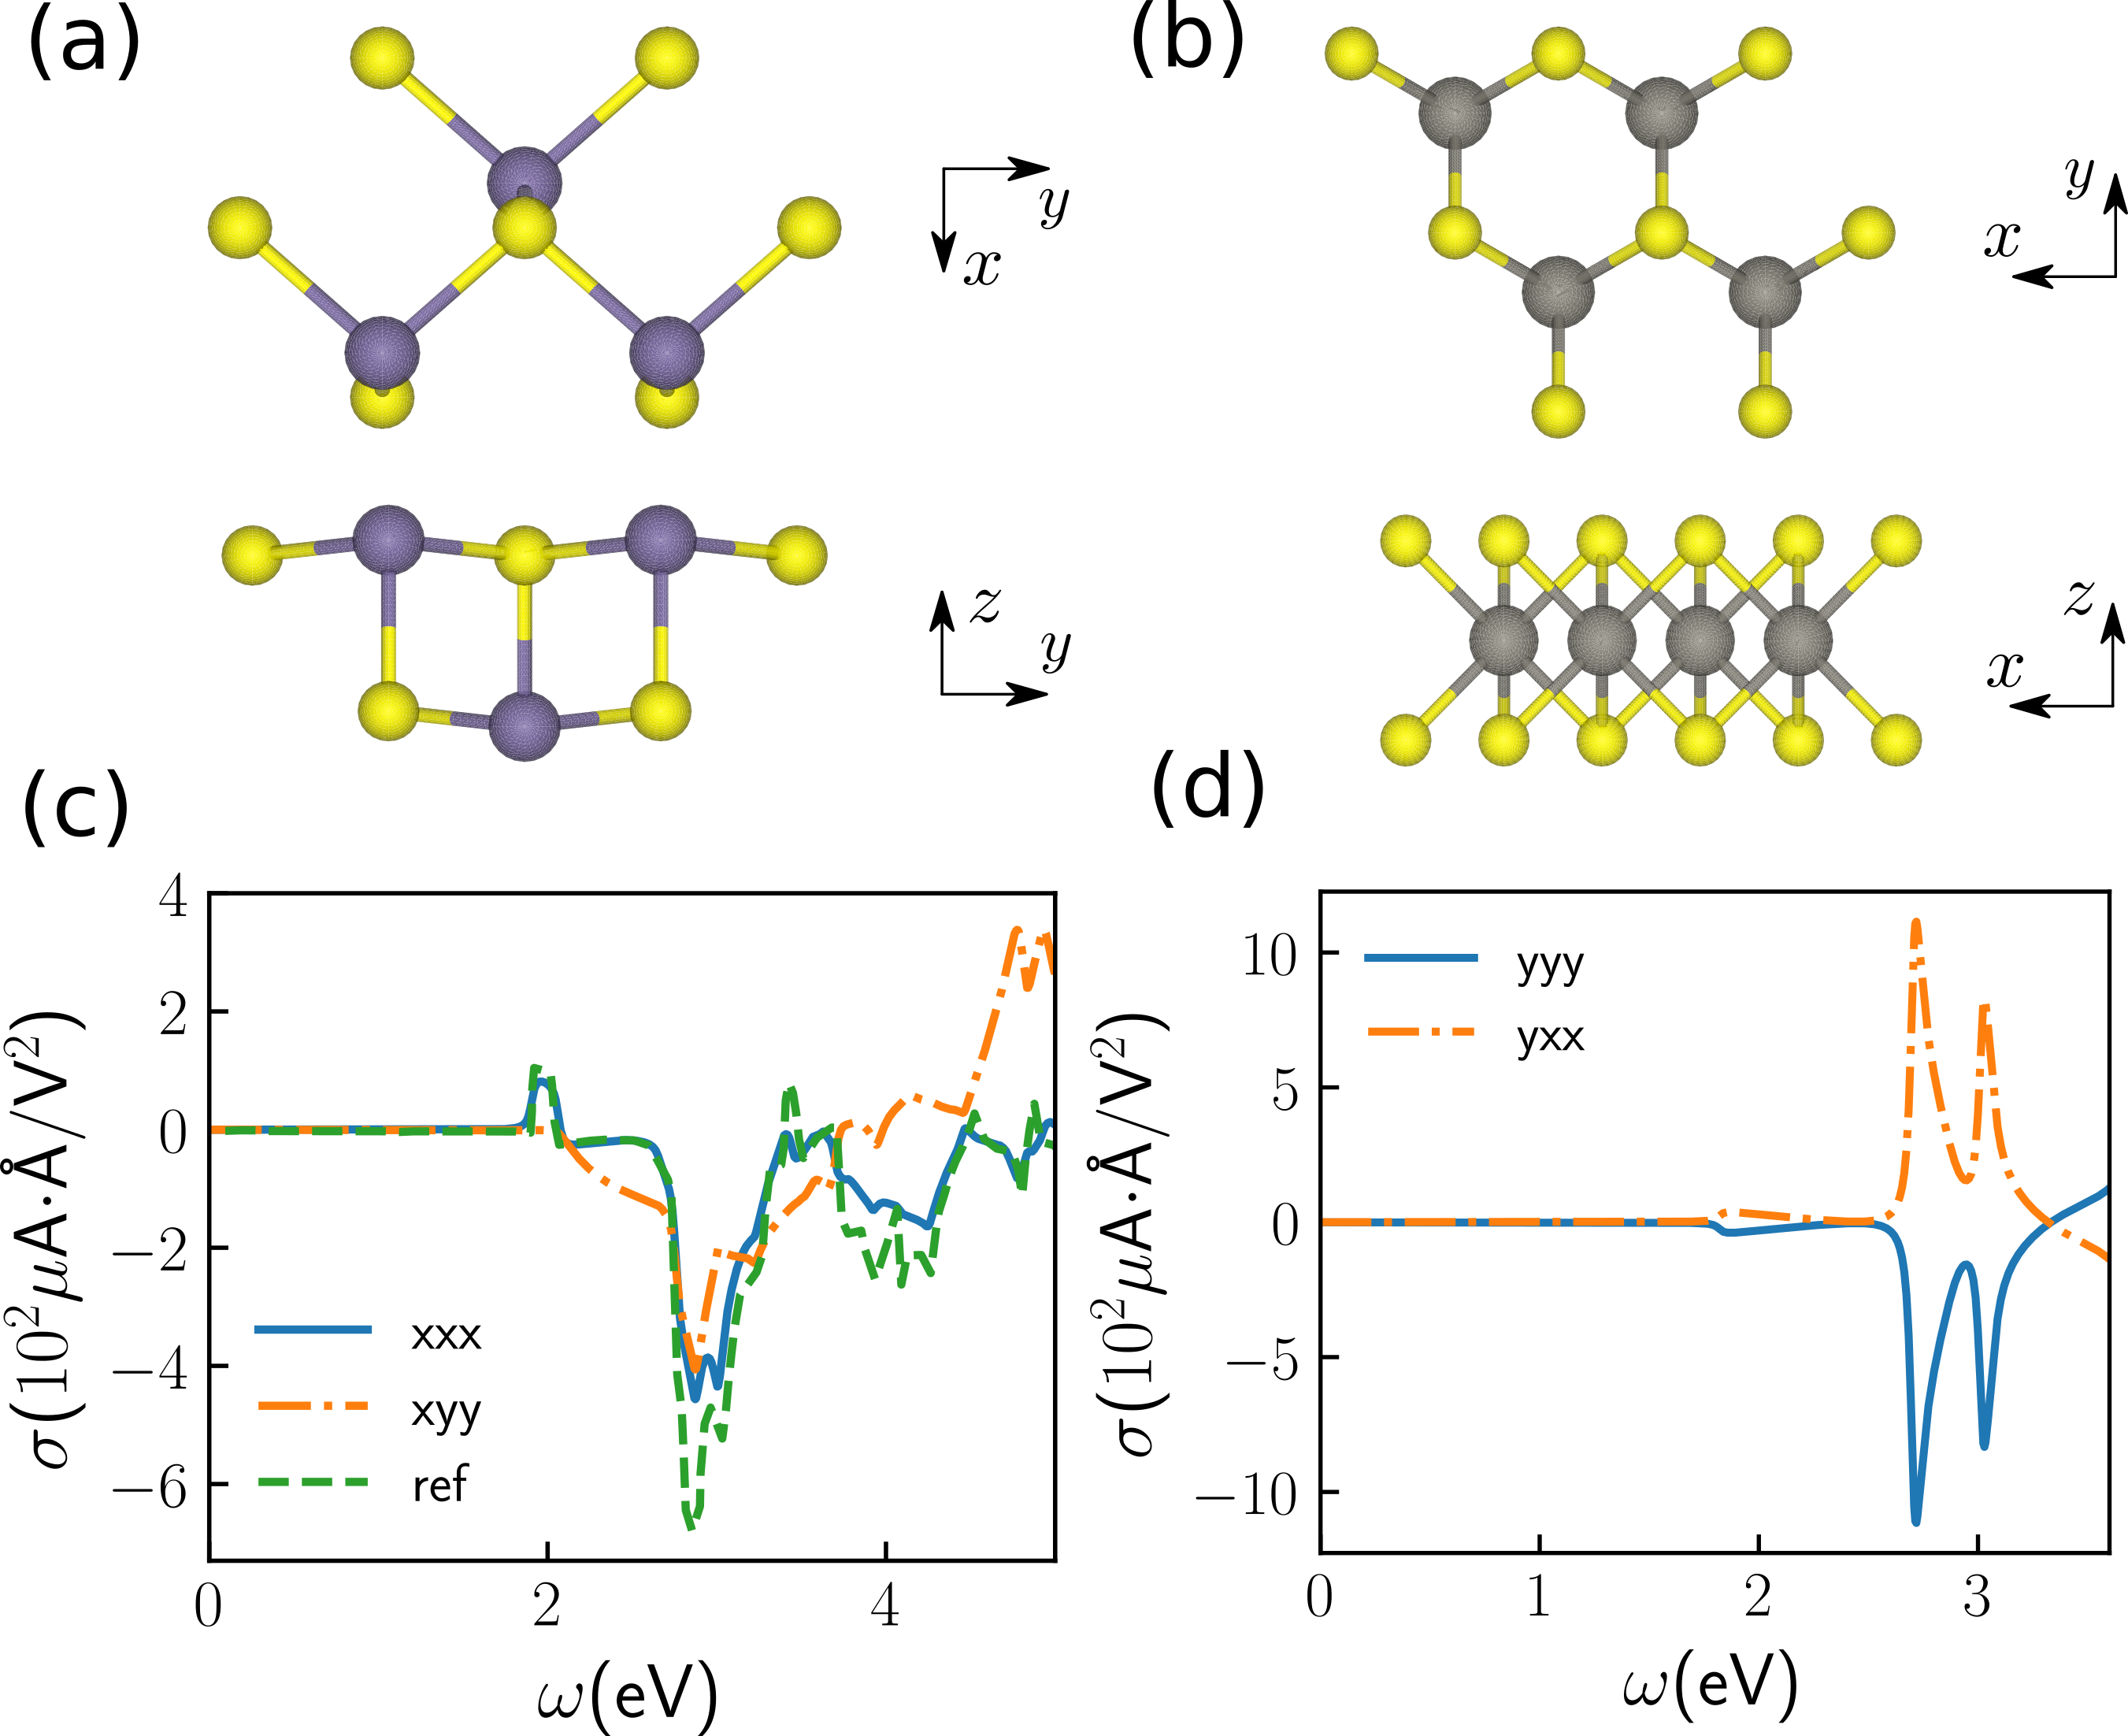
\includegraphics[width=1.0\textwidth]{1.png}
	\par\end{centering}
	\caption{\label{fig1} (a, b)单层GeS【(a)】和WS$_{2}$【(b)】的原子结构的顶视图和侧视图。黄色的小球是S原子,紫色的小球是Ge或者W原子。(c)单层GeS二维位移电导与光频率的关系。文献\onlinecite{rangel_giant_2016}的结果也放了进来。(d)单层WS$_2$的二维位移电流。计算得到的GeS和WS$_2$的带隙分别是1.90 eV和1.82 eV。}
\end{figure}

我们首先来计算二维空间反演破缺的材料GeS和WS$_{2}$的位移电流。之前的研究表明,由于铁电序很大,单层的GeS存在着非常大的位移电流和倍频效应\cite{rangel_giant_2016,panday_strong_2017}。这里,我们使用\textsc{quantum espresso}软件包\cite{giannozzi_quantum_2009},采用\text{pslibrary}投影缀加波的赝势\cite{dal_corso_pseudopotentials_2014}进行计算。电子的交换关联作用采用了Perdew-Burke-Ernzerhof的交换关联泛函\cite{perdew_generalized_1996}来描述。电子波函数采用了平面波基组展开,平面波的截断是60 Ry。我们采用层状模型来模拟二维材料,真空层超过了15 \AA。对于GeS和WS$_2$,我们在布里渊区中的积分分别采用了 $12\times12\times1$和$18\times18\times1$的$k$点。在完成基于密度泛函的第一性原理计算之后,我们采用\textsc{wannier90}软件包\cite{mostofi_updated_2014}构造出了最大局域化Wannier函数。接下来我们采用上述的Wannier插值方法来计算位移电导。计算位移电导的$k$点积分采用了$1000\times1000\times1$的格子,$\delta$函数的展宽取为了$\epsilon = 0.02$eV。值得注意的是,由于二维材料的联合态密度遇到鞍点的时候可以发散,为了避免发散,这个展宽因子是必须的。经过我们的测试,自旋轨道耦合仅仅会稍微改变结果,因此,我们在这里展示没有考虑自旋轨道耦合的结果,方便分析。对于二维材料,我们采用了二维的电流密度的定义$\mathbf{J}_{2D}=\mathbf{J}_{3D}d$,这里$\mathbf{J}_{2D}$是二维电流密度,$\mathbf{J}_{3D}$是超胞计算中的三维电流密度,$d$是超胞在面外方向的长度。在这样的规范下,位移电导变成了$\sigma_{2D}=\sigma_{3D}d$。


单层的GeS存在着一个将$y$变为$-y$的镜面操作$\hat{M}_{y}$。 由于这个镜面操作的存在$\sigma^{xxy}$和$\sigma^{yyy}$都是严格为零的。\fig{fig1}展示了$\sigma^{xxx}$和$\sigma^{xyy}$的结果。文献\onlinecite{rangel_giant_2016}的结果同样展示在了图中。总体上而言,我们的结果和前人的结果吻合的很好。一些峰值定量上的差距可能是计算方法和参数的不同导致的。WS$_2$有着一个将$x$变为$-x$的镜面操作$\hat{M}_{x}$,因此,$\sigma^{xxx}$ 和 $\sigma^{xyy}$被禁戒。WS$_2$的点群$D_{6h}$要求其不为零的位移电导分量$\sigma^{yyy}$和$\sigma^{yxx}$满足如下关系:$\sigma^{yyy}=-\sigma^{yxx}$,这一点在图上也可以看出来。由于带边存在着范霍夫奇点,两种材料的位移电导都在带边存在着小小的跳跃。除此之外,我们看到两个材料高于带隙$1$eV的地方都有几个峰,这些峰都在可见光的范围之内。

\begin{figure}
	\begin{centering}
	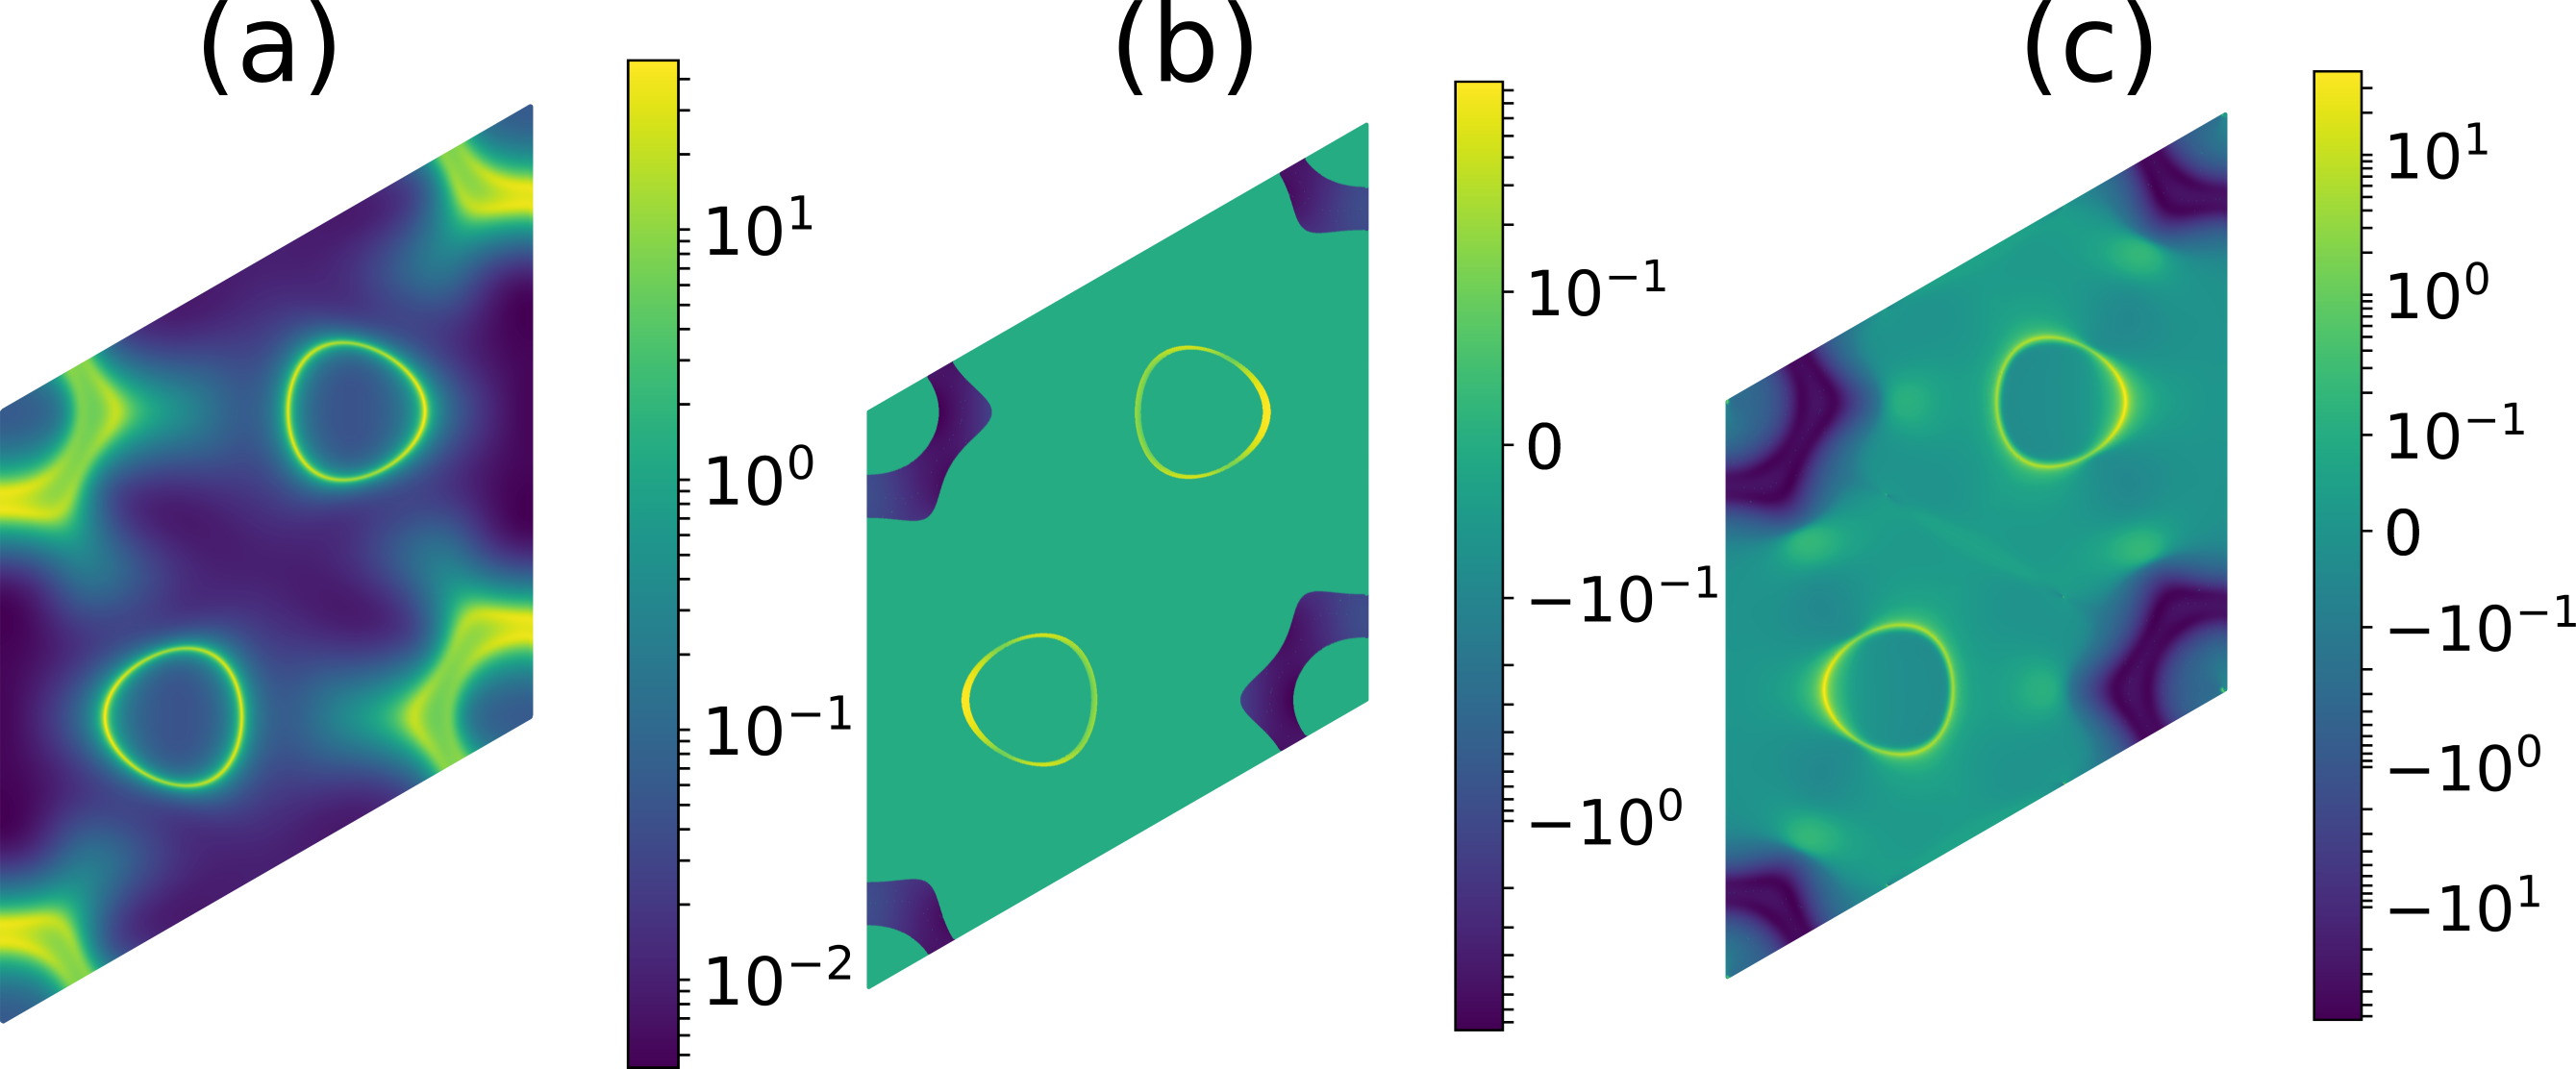
\includegraphics[width=1.0\textwidth]{2.png}
	\par\end{centering}
	\caption{\label{fig2} 单层WS$_{2}$的位移电流的相关量在布里渊区中的分布,我们取光的频率为$2.719$ eV。(a)跃迁速率$r_{nm}^{y}r_{mn}^{y}\delta(\omega_{nm}-\omega)$ (\AA$^{2}$/eV);(b)位移矢量$R_{mn}^{y,y}$ (\AA);(c)位移电导的积分核$r_{nm}^{y}r_{mn}^{y}R_{mn}^{y,y}\delta(\omega_{nm}-\omega)$ (\AA$^{3}$/eV)。}
\end{figure}

为了分析不同的电子态对位移电导的贡献,我们在\fig{fig2}中展示了WS$_2$的位移电导相关的量在布里渊区中的分布,这些量是在位移电导的第一个峰$\hbar\omega = 2.719$ eV处计算的。这些量分别是跃迁速率$r_{nm}^{b}r_{mn}^{b}\delta(\omega_{nm}-\omega)$,位移矢量$R_{mn}^{a,b}$以及他们的乘积。对于时间反演不变的体系:$I^{abb}(\mathbf{k})=I^{abb}(-\mathbf{k})$,这一点可以在\fig{fig2}中看出来。从\fig{fig2}中可以看出两个非常重要的特性:(一)由于狄拉克$\delta$函数的存在,绝大部分$\bk$点对位移电导并没有贡献,只有极少数$\bk$点贡献了非常大的值。因此,布里渊区的积分确实需要大量的$\bk$点才能够收敛。(二)如\fig{fig2}所示,位移矢量大概在$1$\AA 左右,但是在一些地方超过了$10$\AA ,之前的研究\cite{fregoso_quantitative_2016}在模型计算中也注意到了这一点。与此相对,电子的极化的定义可以相差任意一个晶格格矢。要分析位移电导,我们需要完全的理解位移矢量而不是简单的比较导带和价带的电子极化\cite{young2012}。


如前文所述,计算贝里联络的导数可以采用求和规则,而不是二阶微扰的办法,但是这个方法由于需要对所有能带求和,所以并不推荐。除此之外,很多前人的线性响应的计算都采用了紧束缚模型。紧束缚模型可以通过保留第一性原理计算得到的哈密顿量,但是设置$\langle\mathbf{0}n|\hat{\mathbf{r}}|\mathbf{R}m\rangle=\delta_{0\mathbf{R}}\delta_{nm}\mathbf{r}_{n}$得到。\fig{fig3}比较了不同的计算方法得到结果。如\fig{fig3}所示,我们通过设置不同的内窗口和不同的初始投影,得到了两组数目不同的最大局域化Wannier函数,后一组Wanier函数的数目更多一些。\fig{fig3}给出了微扰论和求和规则采用不同组Wannier函数计算得到的位移电导的结果。根据我们的测试,微扰论的计算结果和Wannier的数目并没有什么关系,而求和规则却给出了显然不同的结果。这就展示了求和规则需要对所有能带求和的缺陷。除此之外,两种方法计算得到的位移电导的大小也不太一致,这一点可以有两个解释:(一)求和规则忽略了$\langle n|\partial_{a}\partial_{b}\hat{H}(\mathbf{k})|m\rangle$;(二)对于求和规则来说,Wannier函数的数目尚未收敛;(三)Wannier插值得到的布洛赫波函数仅仅在内窗口和第一性原理重合,因此内窗口外的Wannier插值得到的布洛赫波函数并不是真正的波函数,在求和规则中会产生差异。另外,我们通过忽略位置矩阵元的所有非对角项,得到了紧束缚模型的结果。和微扰论的结果相比,紧束缚的结果有着能够注意到的差异。与此相反,紧束缚模型在计算反常霍尔效应的时候仅仅产生了不到$1\%$的误差\cite{wang_textitab_2006}。我们的结果显示,非线性光学效应比线性响应对波函数的分布更加敏感。

\begin{figure}
	\begin{centering}
	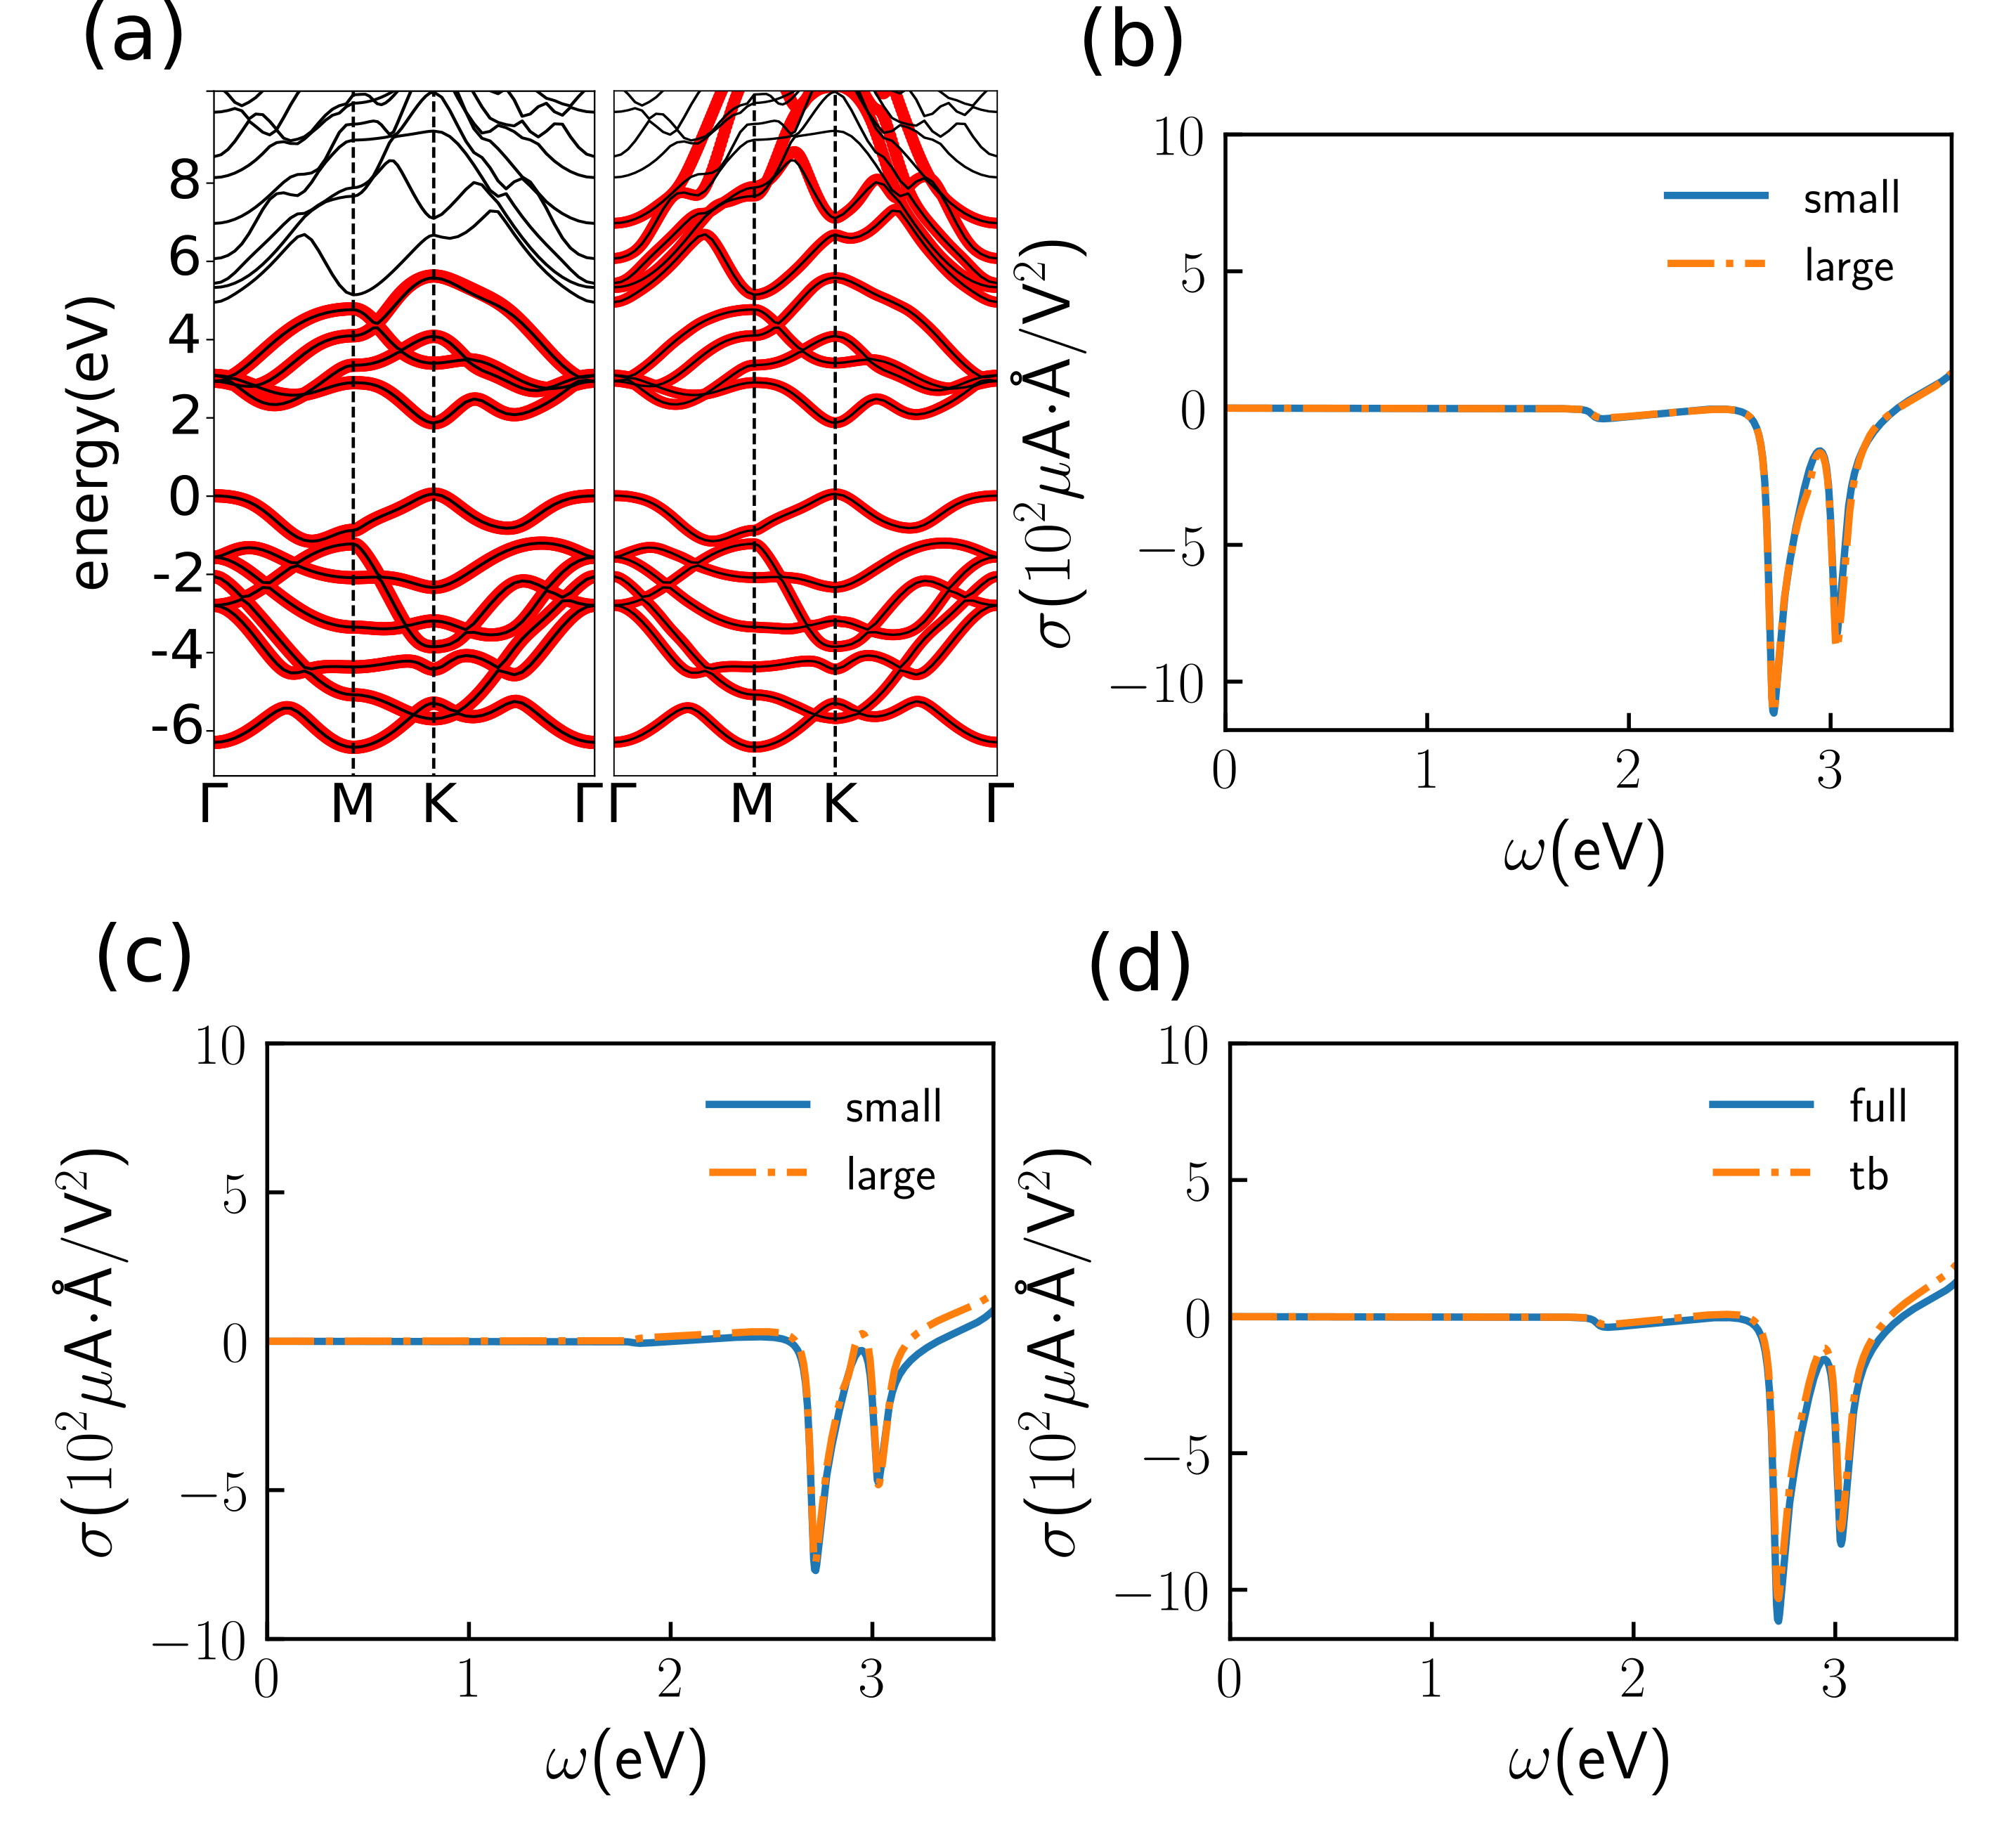
\includegraphics[width=1.0\textwidth]{3.png}
	\par\end{centering}
	\caption{\label{fig3} (a) 单层WS$_2$的能带,黑色线是密度泛函的结果,红色的点是Wannier插值的结果。两幅图对应着两组不同的Wannier函数。左侧的Wannier函数数目较少,在(b-c)中标为了“small”,右侧的Wannier函数数目较多,标为“large”。(b,c) 采用两组不同的Wannier函数的微扰法【(b)】和求和规则【(c)】算得的位移电导。(d) 应用紧束缚【“tb”】和不用紧束缚近似【“full”】计算的位移电导。} 
	
\end{figure}


\subsection{倍频效应}


我们在没有考虑自旋轨道耦合的情况下进行了GaAs的密度泛函计算。在计算中,我们采用了Hartwigsen-Goedeker-Hutter模守恒赝势\cite{hartwigsen_relativistic_1998},Perdew-Burke-Ernzerhof的交换关联泛函\cite{perdew_generalized_1996}以及截断为60Ry的平面波基组。在密度泛函自洽计算中,我们采用了 $6\times6\times6$ 的$\bk$格子,在计算倍频效应的时候,我们采用了 $250\times250\times250$ 的$\bk$格子。考虑到PBE交换关联泛函严重低估带隙,我们采用了两种方式来修正带隙。一种是剪刀修正\cite{nastos_scissors_2005}。剪刀修正指的是假设波函数不变,直接将能量修正为实验带隙。另一种是采用Heyd-Scuseria-Ernzerhof(HSE)杂化泛函\cite{heyd_hybrid_2003}。这两种方法得到的结果展示在\fig{fig4}中。GaAs的实验带隙是$1.42$eV,这要求我们在剪刀修正上加上$0.86$的修正,而HSE的密度泛函计算则给出了稍小一点的带隙($1.25$eV)的带隙。在\fig{fig4}中,倍频效应的虚部在达到二分之一个带隙的时候会开始有值。

GaAs的空间群是$F\bar{4}3m$,这个空间群唯一的非零的倍频系数是$\chi^{xyz}$。这里,我们给出GaAs的倍频系数的结果。剪刀修正和HSE杂化泛函的计算,在峰位和峰型的这些特征上基本一致,但是后一种方法给出了稍微小一点的$\chi^{xyz}$。这两个结果都和前人的计算吻合的很好\cite{rashkeev_efficient_1998,nastos_scissors_2005,hughes_calculation_1996}。我们的计算给出的值稍小一些,可能是因为计算细节上的插值。最后我们说明,我们的结果在用不用紧束缚近似,用不用求和规则的情况下结果都基本相同。这一点证明了我们的方法的可靠性。

\begin{figure}
	\begin{centering}
	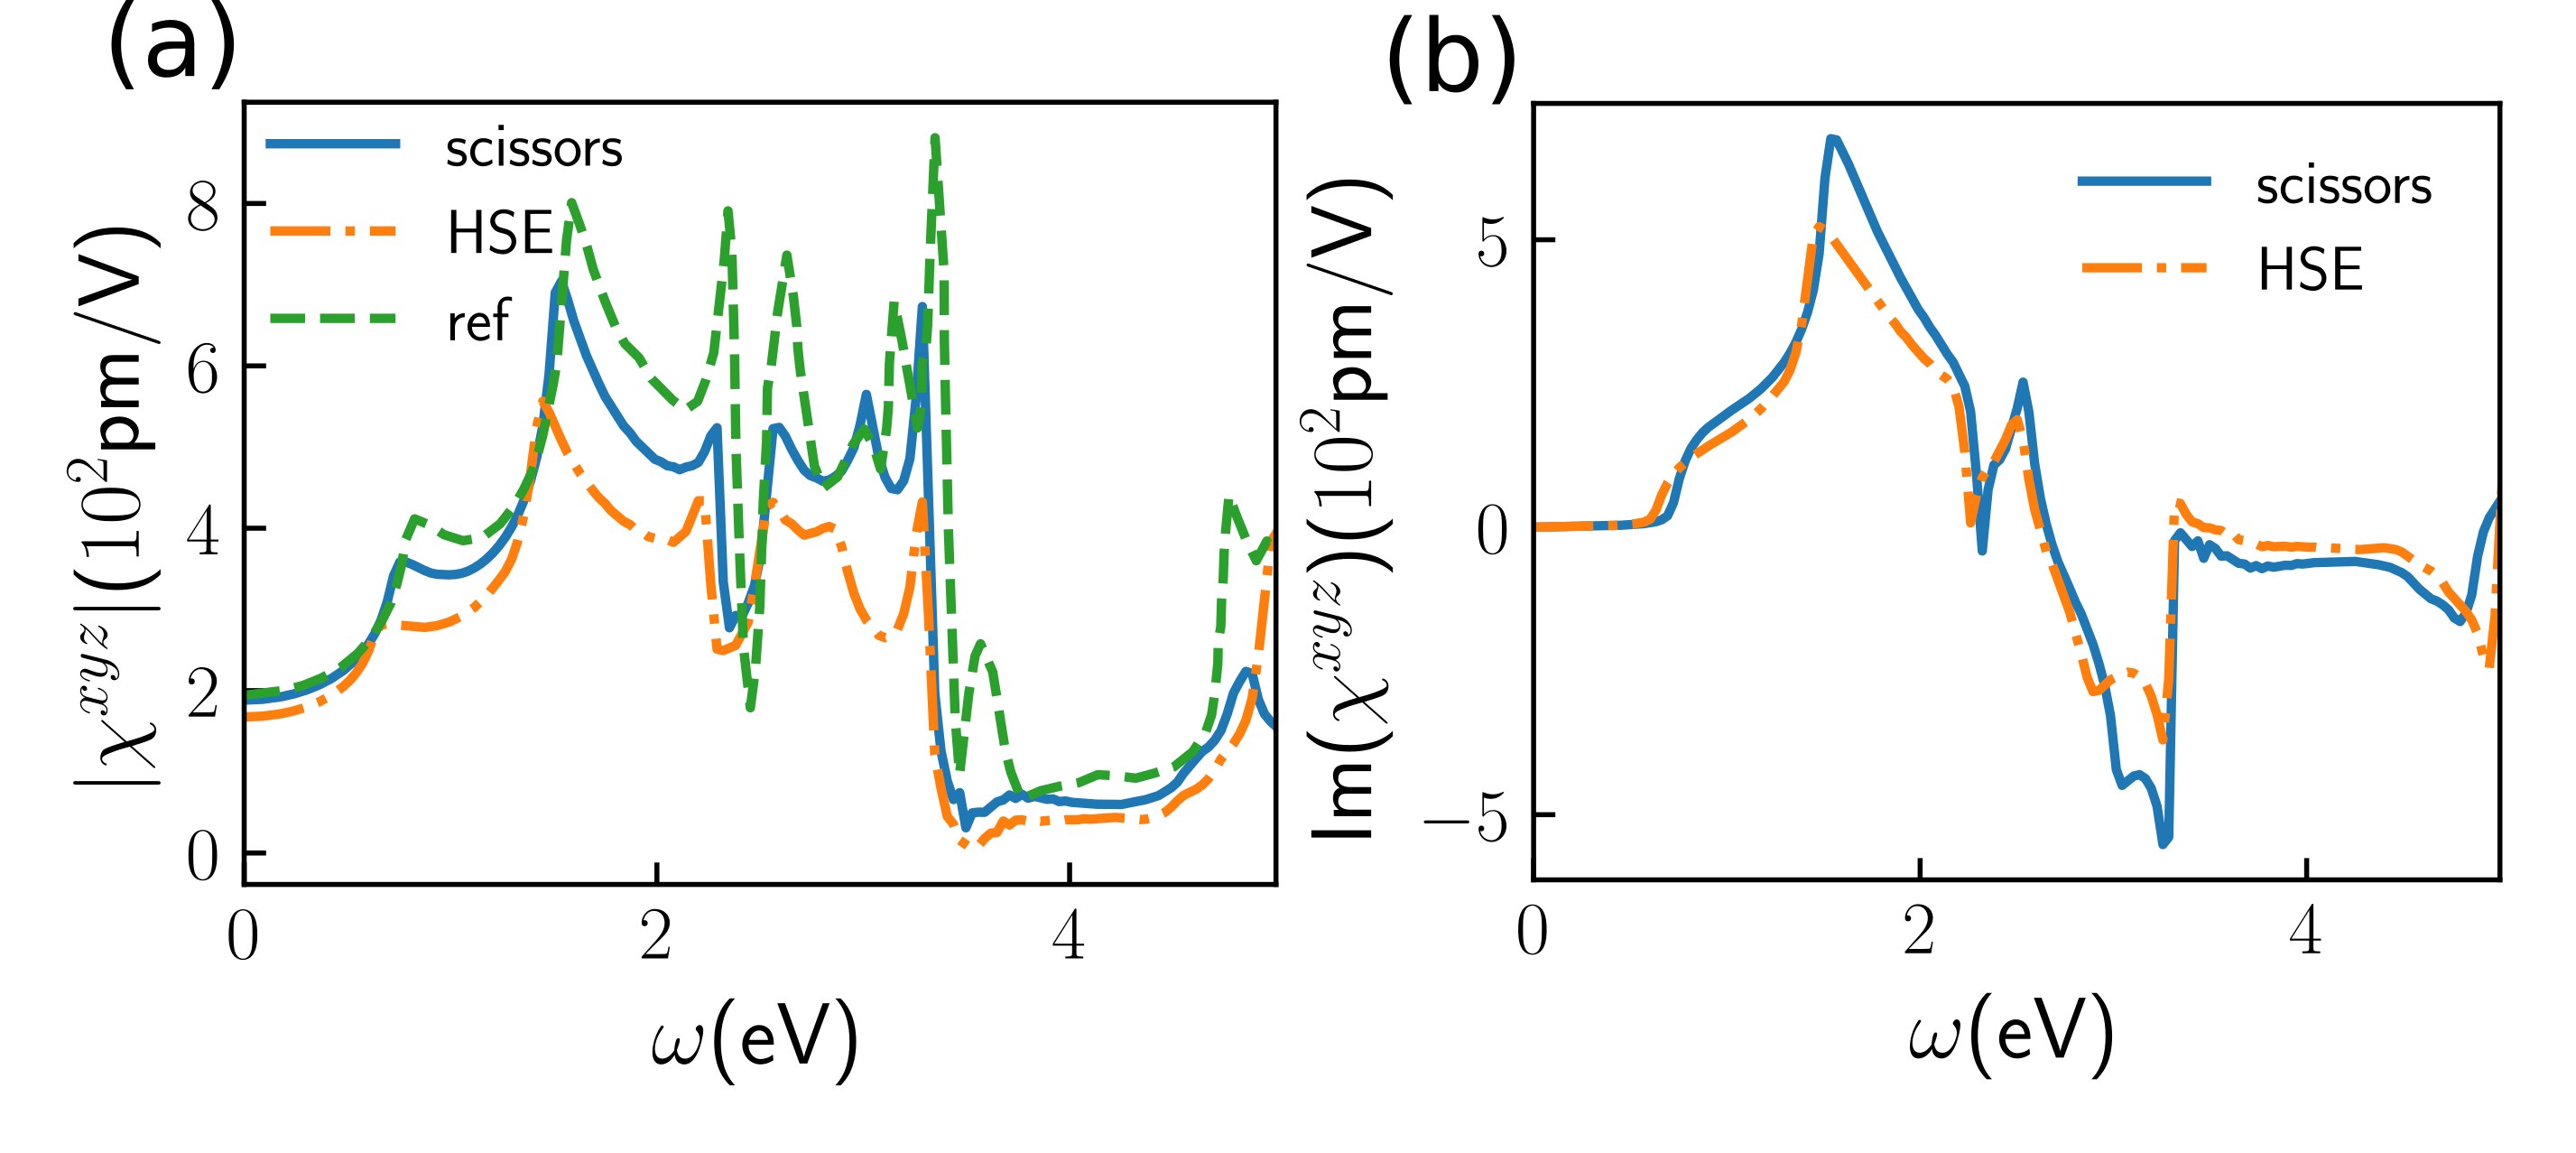
\includegraphics[width=1.0\textwidth]{4.png}
	\par\end{centering}
	\caption{\label{fig4} 采用不同方法计算的GaAs的$\chi^{xyz}$的模【(a)】和虚部【(b)】。(a)图中还画出了文献\onlinecite{nastos_scissors_2005}的结果。}
	\end{figure}
\section{讨论和结论\label{sec:discussions-and-conclusions}}


Wannier插值方法在第一性原理计算中是一个非常重要的工具。Wannier插值方法强大的地方不仅仅体现在计算量很小,也体现在其普适性上。无论是采用密度泛函还是超越密度泛函原理(比如$GW$,杂化泛函等)的第一性原理计算,无论是采用模守恒赝势,PAW赝势还是全电子计算,,无论是包不包括自旋轨道耦合,最大局域化Wannier函数都可以轻松的构造出来。前人的工作展示了Wannier插值方法在对$\bk$点收敛缓慢的线性响应里的应用,我们的工作证明了在非线性效应里面Wannier插值也非常有效。


总结一下,我们提出了一种基于Wannier插值的计算非线性光学效应的手段。我们以位移电流和倍频效应为例展示了这个方法。这个方法首先用\textsc{wannier90}软件包构造出Wannier函数。然后我们利用非线性光学效应的的局域规范不变性,采用微扰论计算任意$\bk$点相关的矩阵元,例如贝里联络及其导数。在位移电流和倍频效应之外,我们的方法还可以直接应用于其他的非线性光学效应,比如和频差频效应,以及克尔效应。我们的方法应该还可以推广三阶以及更高阶的光学效应的计算上。

为了证明我们方法的可靠性,我们计算了单层GeS和WS$_{2}$的位移电流和GaAs的倍频效应。我们在Wannier插值中也尝试了传统的计算贝里联络的求和规则并且和微扰论进行了比较。我们发现由于不需要对所有能带求和,基于微扰论的方法更加有优势。另外,我们也测试了紧束缚方法,紧束缚方法不需要知道 $\langle\mathbf{0}n|\hat{\mathbf{r}}|\mathbf{R}m\rangle$的非对角项。在线性响应中,紧束缚近似的结果和完全第一性原理的结果几乎相同,但是在非线性光学效应中,紧束缚近似则会造成结果有一些可以观测到的差别,这表明了非线性光学效应对波函数的分布更加敏感。我们认为Wannier插值将会成为第一性原理计算非线性光学效应中的用途广泛,功能强大的工具。
